\documentclass[reqno]{amsart}


\pagestyle{empty}

\usepackage{graphicx}
\usepackage[margin = 1cm]{geometry}
\usepackage{color}
\usepackage{cancel}
\usepackage{multirow}
\usepackage{framed}
\usepackage{algorithm}
\usepackage{algorithmic}
\usepackage{amssymb}
\usepackage{stackengine}


\newtheorem{thm}{Theorem}
\newtheorem{cor}{Corollary}
\theoremstyle{definition}
\newtheorem{definition}{Definition}

\newenvironment{handwave}{%
  \renewcommand{\proofname}{Handwavey proof}\proof}{\endproof}
  %\renewcommand{\qedsymbol}{$\blacksquare$}

\begin{document}
\begin{flushleft}
{\sc \Large AMATH 301 Rahman} \hfill Week 4 Theory Part 2
\bigskip
\end{flushleft}

\newcommand{\R}{\mathbb{R}}
\newcommand{\N}{\mathbb{N}}
\newcommand{\Z}{\mathbb{Z}}
\newcommand{\Q}{\mathbb{Q}}
\renewcommand{\CancelColor}{\color{red}}
\newcommand{\?}{\stackrel{?}{=}}
\renewcommand{\varphi}{\phi}
\newcommand{\card}{\text{Card}}
\newcommand{\bigzero}{\text{\Huge 0}}
\newcommand{\curvearrowdown}{{\color{red}\rotatebox{90}{$\curvearrowleft$}}}
\newcommand{\curvearrowup}{{\color{red}\rotatebox{90}{$\curvearrowright$}}}



\section*{Week 4 Part 2:  Eigenvalues and Eigenvectors}

Thus far we have talked about matrices as arrays.  But how do we use this in Science?  Lets think about matrices as transforms.  A transform takes a vector in one space, applies the properties of another space, and shows us what the vector looks like in the second space.

For example, suppose everything in Country B costs 5 times as much as things in Country A.  If something costs x in A it costs 5x in B, where we are thinking of the scalar variable x as a one element vector.

This concept becomes much more powerful with matrices where we can stretch, squeeze, twist, and turn vectors in several dimensions.

For example, say we have the vector $v = (1, 1)$ and a matrix
%
\begin{equation*}
A = \begin{bmatrix}
2 & -1\\
1 & -1/2
\end{bmatrix}
\end{equation*}
%
The vector $v$ is the velocity of a rocket in the vacuum of space.  The matrix $A$ contains the atmospheric and gravitational properties of a certain planet.  If the rocket does everything the same on the planet as it did to get a velocity of $v$ in space, the vector $Av$ would be the velocity on the planet.  Further, $A$ is called the {\color{red}\underline{linear transform}}.  We can see this in the figure below
%
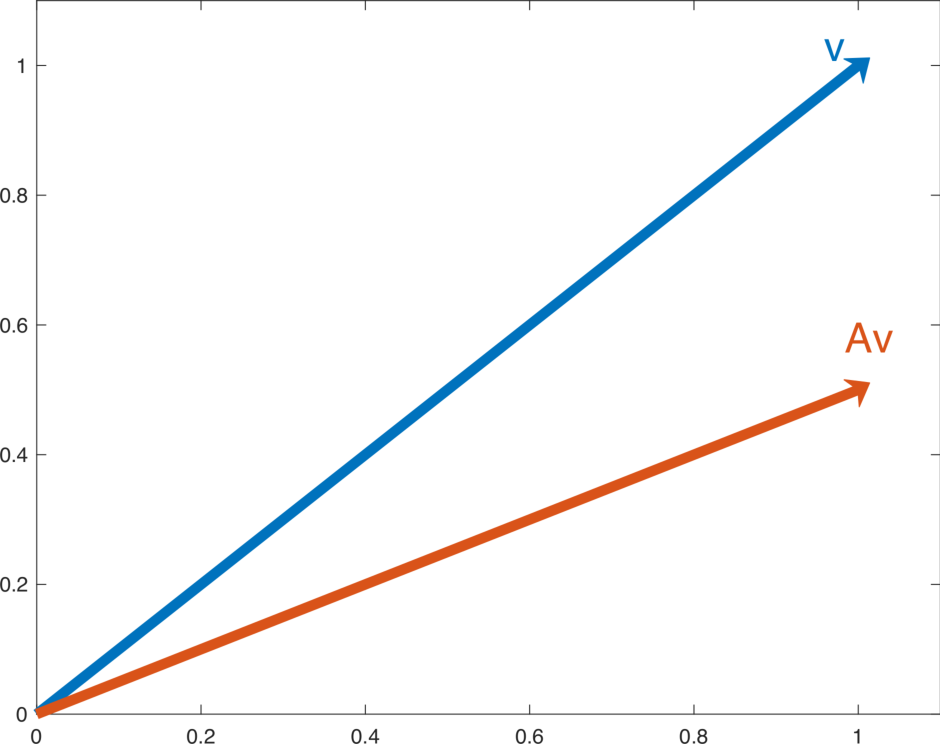
\includegraphics[width = 0.7\textwidth]{Transform}

Often in science we look for invariant: things that don't change with external stimuli.  That is what an eigenvector is.  It might stretch or compress, but it stays true to its course.  The stretching/compressing is determined by the eigenvalue.

This can be written mathematically as $Ax = \lambda x$, where $\lambda$ are called the \underline{eigenvalues} and $x$ are called the \underline{eigenvectors}.  Interestingly, eigenvalues and eigenvectors completely describe a transform.  This is also used in ODEs to solve them.

{\color{red} How do we solve for $\lambda$ and $x$?}  Lets move some terms around and see what we get.
%
\begin{equation*}
Ax = \lambda x \Rightarrow (A-\lambda I)x = 0 \Rightarrow \det(A-\lambda I) = 0 \quad \text{if $x\neq 0$}.
\end{equation*}
%
We don't want the trivial solution $x=0$ because that does not tell us anything about the problem.
After finding the determinant we solve for the roots of the polynomial that arises from the determinant, which are the eigenvalues, $\lambda$.  Then we find $x \in \mathcal{N}(A-\lambda I)$ ($x$ is in the nullspace of $A-\lambda I$), which are the eigenvectors.

\pagebreak

Lets look at a few examples.

\begin{enumerate}

\setlength{\itemsep}{2em}

\item[Ex:  ]  Solve the eigenvalue problem
%
\begin{equation*}
\begin{bmatrix}
4 & 1\\
3 & 2
\end{bmatrix}x = \lambda x.
\end{equation*}
%

\textbf{Solution:  }  We first compute $\det(A-\lambda I)$ and solve for $\lambda$,
%
\begin{equation*}
\Rightarrow \begin{vmatrix}
4-\lambda & 1\\
3 & 2-\lambda
\end{vmatrix} = (4-\lambda)(2-\lambda) - 3 = 8 - 6\lambda \lambda^2 - 3 = \lambda^2 - 6\lambda + 5 = (\lambda - 5)(\lambda - 1) = 0 \Rightarrow \lambda_1 = 5,\, \lambda_2 = 1.
\end{equation*}
%
Next we solve for the eigenvectors.  For $\lambda_1$,
%
\begin{equation*}
A - \lambda_1I = \begin{pmatrix}
-1 & 1\\
3 & -3
\end{pmatrix}x_1 = 0 \Rightarrow x_1 = \begin{pmatrix}
1\\
1
\end{pmatrix}
\end{equation*}
%
For $\lambda_2$,
%
\begin{equation*}
A - \lambda_2I = \begin{pmatrix}
3 & 1\\
3 & 1
\end{pmatrix}x_2 = 0 \Rightarrow x_2 = \begin{pmatrix}
1\\
-3
\end{pmatrix}
\end{equation*}
%
It should be noted that the eigenvectors don't have to be those exact vectors.  They just have to be any vectors that satisfy the eigenvalue equation.

\item[Ex:  ]  Solve the eigenvalue problem
%
\begin{equation*}
\begin{bmatrix}
1 & -1\\
1 & 1
\end{bmatrix}x = \lambda x.
\end{equation*}
%

\textbf{Solution:  }  We first compute $\det(A-\lambda I)$ and solve for $\lambda$,
%
\begin{equation*}
\begin{vmatrix}
1 - \lambda & -1\\
1 & 1-\lambda
\end{vmatrix} = 1 - 2\lambda + \lambda^2 + 1 = \lambda^2 - 2\lambda + 2 = 0
\Rightarrow \lambda = \frac{1}{2}\left(2 \pm \sqrt{4 - 8}\right) = 1\pm i.
\end{equation*}
%
Next we solve for the eigenvectors.  For $\lambda_1 = 1 + i$,
%
\begin{equation*}
A - \lambda_1I = \begin{pmatrix}
-i & -1\\
1 & -i
\end{pmatrix}x_1 = 0 \Rightarrow x_1 = \begin{pmatrix}
i\\
1
\end{pmatrix}
\end{equation*}
%
For $\lambda_2 = 1 - i$,
%
\begin{equation*}
A - \lambda_2I = \begin{pmatrix}
i & -1\\
1 & i
\end{pmatrix}x_2 = 0 \Rightarrow x_2 = \begin{pmatrix}
i\\
-1
\end{pmatrix}
\end{equation*}
%
Notice that these eigenvectors are complex conjugates because the eignevalues are complex conjugates, so we only have to have to solve for one eigenvector and get the other one for free.

\end{enumerate}

\pagebreak

Anyone interested in higher dimensional eigenvalue problems, you can continue below

\begin{enumerate}

\item[Ex:  ]  Solve the eigenvalue problem
%
\begin{equation*}
\begin{bmatrix}
1 & 6 & 0\\
0 & 2 & 1\\
0 & 1 & 2
\end{bmatrix}x = \lambda x.
\end{equation*}
%

\textbf{Solution:  }  We first compute $\det(A-\lambda I)$ and solve for $\lambda$,
%
\begin{equation*}
\begin{vmatrix}
1-\lambda & 6 & 0\\
0 & 2-\lambda & 1\\
0 & 1 & 2-\lambda
\end{vmatrix} = (1-\lambda)(4-4\lambda + \lambda^2 - 1) = (1-\lambda)(\lambda - 3)(\lambda - 1) = 0
\Rightarrow \lambda_1 = 1,\, \lambda_2 = 1,\, \lambda_3 = 3.
\end{equation*}
%
Then our eigenvectors are
%
\begin{equation*}
\begin{bmatrix}
1 - \lambda & 6 & 0\\
0 & 2-\lambda & 1\\
0 & 1 & 2-\lambda
\end{bmatrix}x = 0 \Rightarrow x_1 = \begin{pmatrix}
1\\
0\\
0
\end{pmatrix} = x_2,\, x_3 = \begin{pmatrix}
3\\
1\\
1
\end{pmatrix}
\end{equation*}

\item[Ex:  ]  Solve the eigenvalue problem
%
\begin{equation*}
\begin{bmatrix}
1 & -1\\
1 & 1
\end{bmatrix}x = \lambda x.
\end{equation*}
%

\textbf{Solution:  } We first compute $\det(A-\lambda I)$ and solve for $\lambda$,
%
\begin{equation*}
\begin{vmatrix}
4-\lambda & -5\\
2 & -3-\lambda
\end{vmatrix} = (4-\lambda)(-3-\lambda) + 10 = \lambda^2 - \lambda - 2 = (\lambda - 2)(\lambda + 1) = 0 \Rightarrow \lambda_1 = 2,\, \lambda_2 = -1.
\end{equation*}
%
Then our eigenvectors are
%
\begin{equation*}
\begin{pmatrix}
4-\lambda & -5\\
2 & -3-\lambda
\end{pmatrix}x = 0 \Rightarrow x_1 = \begin{pmatrix}
5\\
2
\end{pmatrix},\, x_2 = \begin{pmatrix}
1\\
1
\end{pmatrix}
\end{equation*}

\end{enumerate}


\end{document}